\documentclass{article}
\usepackage{graphicx}


\begin{document}
\title{Technical Document}
\date{\today}
\author{Kyle Chuang}
%  \maketitlepage

%  \newpage
\section{General Overview}
There has been an extensive literature and debate on hotspots in traffice analysis. Our proposed hotspot analysis using hdbscan algorith is unique and different amongst commonly accepted measures of fatalizes/mile across roadways. Fatalities/mile may have a difficult time taking into account the features of the crash while our algorithm focuses specifically on those different features. This allows the user to focus on what is more likely to be connected to crashes and diagnose potential solutions for the area.

Further difficulties in hotspot detection stem from the variability of traffic. As hotspots may randomly disappear from 1 year despite appearing n all other years, we provide a method to find the hotspot that appear across time.

\section{Clustering Algorithm Selection}
The are many clustering algorithms available. The most popular algorithms include K-Nearest Neighbors (KNN), K-Means and Gaussian Mixture Models (GMM). Unfortunately, those popular algorithms were not suitable for the problem posed. For KNN/K-means, the weakness stems from stability. Multiple runs are typically required to assess stability and there are no guarantees of stability within each run for any given data point. For GMM and K-means, the spherical/elliptical constraints for each cluster may not be appropriate for a traffic analysis problem as hotspots may run along an unconstrained road or a geographic feature. Finally, the clustering algorithms provided above are unable to classify points as "not in cluster". Even with modified method of "cutting" off points at a given distance/probability (K-mean/GMM) as unclustered, other weaknesses make the algorithms provided inapproriate for the analysis.

\section{HDBScan}
HDBScan (hierarchical density based scan) was chosen as the clustering algorithm. HDBScan is a clustering algorithm based on density. It is non-parametric and shapewise unconstrained. The algorithm is also consistent and stable. Repeated runs of the algorithm will always provide the same results unlike some of the algorithms above. Additionally, it can classify data points as not in any cluster based on cluster stability and density.  HDBScan can succintly be described as clustering based on how close the data points are relative to each other in a given area.

HDBScan begins by taking $n$ samples all points. The $n$ sample circlular space radius is called the core distance. After the core distances has been determined, the algorithm computes the reachability for all data points. Reachability is defined as the maximum distance between the 2 point or core distance. A hierachical tree is built based on reachability metric. Clusters are determined based on stability of the parent tree structure compared to the children node tree structure\footnote{For a more detailed discussion, please refer to the following link -  https://hdbscan.readthedocs.io/en/latest/how\_hdbscan\_works.html.}

\section{Methodology}
The clustering methodology based on HDBScan can be described as follows:
\begin{enumerate}
	\item Perform the clustering for each year from the algorithm below (yearly clustering algorithm).
	\begin{enumerate}
			\item Select all the points where the variable of interest is active and drop all the other points. For example, select all data points where the driver is drowsy and drop all the other data points.
			\item Cluster the selected points based on geographic location using the manhattan distance metric.
			\item Create a polygon (convex hull) from each clusters found to determine the problem area.
			\item Label all data points to belong to cluster $x$ if they are inside the boundaries of polygon $x$.
			\item Perform a significance test for all point inside a cluster polygon against all unclustered points. A $p-value$ of 0.05 is determined to be significant. If a cluster is not found to be significant, it is relabeled as unclustered.\footnote{The significance test used was the wilcoxon ranked sum test. This was chosen over t-test since it was non-parametric. To satisfy the normality constraint of the t-test, hundreds of data points were required. The number of data points and normality was empirically determined using sampling and the shapiro-wilks normality test. The $\chi^2$-test was not chose since the data was always symmetric.}
	\end{enumerate}
	\item Once all years has been clustered, overlay the cluster polygons on top of each other geographically. Find the intersections of all polygons that overlap more than $n$ years. The intersections are now time-based cluster polygons.
	\item Relabel all points based on time-based cluster polygons for cluster determination.\footnote{The time-based cluster polygons were expanded by 0.01\% (approximately 1/2 mile in distance) to ensure the inclusion of the polygon vertices itself. The alternative was to iterate through the entire dataset and check for the points on the vertices/edges. This was done to improve the computational speed for efficient visualization.}
	\item Perform a significance test for all points inside time-based cluster polygons against all unclusterd points. If time-based cluster polygon is not found to be significant, the points are relabeled as unclustered.
\end{enumerate}
From a statistical perspective, the yearly clustering algorithm should identify a false positive cluster only 1 out of 20 times if random points from that particular year's dataset to form a a cluster. The false positive cluster rate for time-based polygon clusters will be the same assuming random points are selected from all available years.

An example is provided below using an intersection of 2 years. Each colored polygon is a significant cluster polygon for each individual year. However, only the red colored data points are significant clusters across time.
\begin{center}
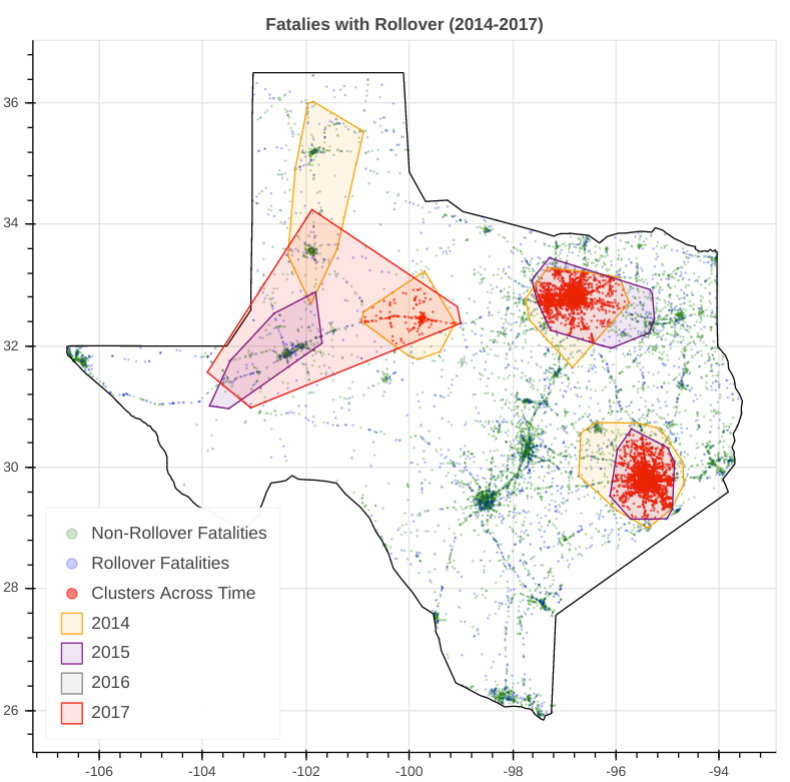
\includegraphics[scale=0.4]{technical.png}
\end{center}
\end{document}


